\chapter{}

Life was, as expected, substantially easier during the week now that we no longer had to work
around the hip spica. The first couple of days of classes, Monique fielded dozens of questions
about her new, much lesser immobilization.

During the first week of the short leg cast and camwalker, she still used the wheelchair. She
retold the same story she'd told at the restaurant- how she could use crutches as long as there
was no pain, but added that she was being careful away from home. She said she didn't want to
start hurting and be forced to stay on her feet. She told people that she was so glad to be free
of the body cast and getting closer to normal, that she did not want to chance a setback. She'd
follow orders to the letter to keep her healing progressing.

At home in the evenings, Monique exercised quite a bit. Even with the camwalker off, the short
leg cast on her left leg kept her from anything too strenuous, but she did what she could to
regain muscle tone and flexibility.

The car show in Illinois we planned to attend was coming up in just a few days, and on
Thursday, we started making our plans and preparations for the weekend. After classes were
finished, we headed to a couple of the shops near our house that sold retro style clothing. At
the traditional car shows, many attendees ``dress the part,'' and we decided to do the same. We
picked up a bowling shirt and a porkpie hat for me, and Monique looked at some vintage dresses,
but eventually decided on an older style halter top. To go with it, she picked out a new pair of
jeans. All of her jeans have that great faded look, but for the show, she wanted a pair of dark,
non-faded jeans. To accessorize, she also picked out a belt with a large, fancy buckle, and an
oversized pair of sunglasses.

\aside{One more accessory I'll need, but that one is sitting in the casting room at home,} she
thought to herself.

Back home, over dinner, we discussed the final plans. After her last class on Friday, we would
cut her out of the cast, then pack some clothes and take off. We would find a hotel for Friday
and Saturday nights, which would allow us to get to the show early, and stay late. We'd drive
back on Sunday afternoon, then get her into a new cast before bed.

``Can we do one more thing before we leave?'' Monique asked.

``What's that?'' I said.

She smiled. ``Well, plaster is pretty retro. It would really add to the ensemble if I had a
cast.''

``What do you have in mind?''

``Well, we will be walking all day,'' she said. The walking will be good for me, and I don't
want anything hindering me. How about an arm cast?''

``It has been a while since you had an arm cast.'' I said. ``But I get to choose. If I let you
decide, you'll probably pick a double shoulder spica,'' I said with a smile.

Friday afternoon, we went home and immediately set our preparations into motion. We went
straight to the casting room, where she took off her camwalker while I got the saw ready. I cut
her left leg free from the cast, and she walked around the room for a few minutes, loosening up
her ankle. We packed our bags, and loaded them into her Expedition, then headed back into the
cast room.

With Monique seated on the casting table, I slipped off her top, and draped a drop cloth
around her torso to protect from plaster splatter. I cut a length of three inch stockinette to
length, and then cut a slit for her thumb. I unrolled it on her left arm, where it ended just
past the elbow. I then took a six inch long piece of two inch stockinette and slit it from both
ends almost all the way to the center. I slid this over her thumb and let one set of tails wrap
around her hand and wrist, while I taped the other tails over her thumb for the time being.

\begin{thought}
Monique watched him work, wondering what this cast was going to be. When he said it was
something he hadn't done before, she'd suspected a cylinder arm cast, but this was definitely
not going to be a cylinder. Whatever it was to be, she was enjoying the feel and the sight of
the application.
\end{thought}

I continued by wrapping padding over her arm from the knuckles of her hand to just barely past
her elbow, making sure to trim the padding around the thumb with scissors to prevent too much
buildup in the web area.

When the padding was complete, I took a roll of four inch plaster and unrolled, it, folding it
over itself until I had a nice splint about two feet long. I dipped it, wrung it out, and
wrapped it around her elbow so that the ends stopped evenly with the thumb. I held it in place
with one hand while I dipped a roll of three inch plaster, and began wrapping her arm to hold
the splint in place.

``A sugar tong cast!'' Monique said. ``Very rare. Very cool.''

``Mmm Hmm,'' I said, focused on my work.

As I wrapped her arm with the three inch roll, I snipped the plaster with my scissors as it
passed through the web of her hand. I wanted her to have plenty of movement in her thumb and
hand, while keeping the wrist immobile.

When I finished with the first roll of plaster, I gave it a quick smoothing, then folded the
stockinette and padding back at her fingers. I pulled it back enough to give a good, though not
complete, range of motion in the last joint of the hand before the fingers. I then untaped the
tails of the stockinette over her thumb, and wrapped the tails back around her hand and wrist. I
could see that she'd also have a good range of motion in the thumb, as I had wanted. I then
pulled the stockinette from her upper arm back until it was even with her elbow, making a slit
to allow it to lay flat.

I finished the cast with a final roll of three inch plaster, smoothing it as I went, making
sure to keep the fingers and thumb mostly free. I smoothed it out and molded it by pressing
slightly on the palm of her hand until the plaster had taken a set. At this point, I buffed it
out with a damp cloth, and we waited for it to dry enough to travel.

The evening drive to Illinois was enjoyable. Once we'd cleared Louisville, the Friday evening
rush hour traffic became lighter. Whenever we're travelling, we always hold hands, and holding
her casted left hand made the drive that much more enjoyable. Once we were near the show, we
noticed that every hotel parking lot was packed with old cars. We saw everything from gorgeous
customs to rusty rat rods. This was going to be a big show. We found our hotel, checked in, then
went out for a late meal before retiring for the night.

The show was amazing! There were acres and acres of shiny, ground scraping customs, faded
original survivor cars, hot rods with their engines exposed, and rat rods that looked like you'd
need a tetanus shot after driving them. In addition, there was a stage with great live
rockabilly music all day long, a swap meet with cars and parts for sale, and vendor booths with
everything from new parts for cars to vintage clothing and accessories. And, of course, there
was plenty of food and beer available.

We registered Monique in the pinup girl contest, and set out to take in everything that the
show had to offer. I really enjoy all of the cars, though some of the rat rods were bordering on
ridiculous and downright unsafe. We took photos, talked about most of the cars, and talked with
many of the owners about their cars. I tend to prefer the hot rods and the wilder customs from
the late 1940's and early 1950's, while Monique seemed most fascinated with the bigger cars from
the late 1950's and early 1960's.

\begin{thought}
Monique had been to car shows before, but nothing like this one. This show seemed to be
populated by blue collar people who built their own cars, instead of people with money who paid
others to build their cars for them. These people seemed more real. The music and atmosphere of
the show just made everything about the day enjoyable.
\end{thought}

At 4:00 pm, there was a break in the music as the contest for the pinup girls was held.
Monique and the others went up on stage and each took their turn strutting out to center stage
amid the cheers, whistles and catcalls. Afterward, they announced the results, and Monique
placed second.

As the evening approached, the bands kept getting better and wilder, and the beer flowed more
freely. The crowd got louder and rowdier, but never got out of hand. We headed back to the hotel
late, and collapsed into bed. Between all of the walking, the sun and the beer, we were asleep
almost as soon as our heads hit the pillows.

We slept in on Sunday, and headed home in the afternoon. When we arrived, I cut Monique out of
her arm cast, and then applied a fresh short leg cast to her left leg.

Once it was fully dry, we went to the computer, where I uploaded the pictures from the camera,
and we looked through them for awhile, reliving the memories of the day before. Before long,
Monique excused herself to bed, while I kept looking through the photos. One particular photo
was rather striking: It was a picture of Monique standing, cigarette in hand, next to a custom
Chevrolet. She had posed with a stance and expression as though she were incredibly bored. I
liked the picture so much that I got paper and pencil and did a sketch of it.

All week, Diane had gone to the statue, hoping to maybe see Monique. She had a lot of
questions to ask: ``Why hadn't she told her about being hurt?  Why had she lost touch
completely?'' And, since learning that Quinn might be the new boyfriend, a new question was
bothering her: ``Was Monique really hurt, or was this all faked as a part of Quinn's `art?'\,''
\newpage
\begin{center}
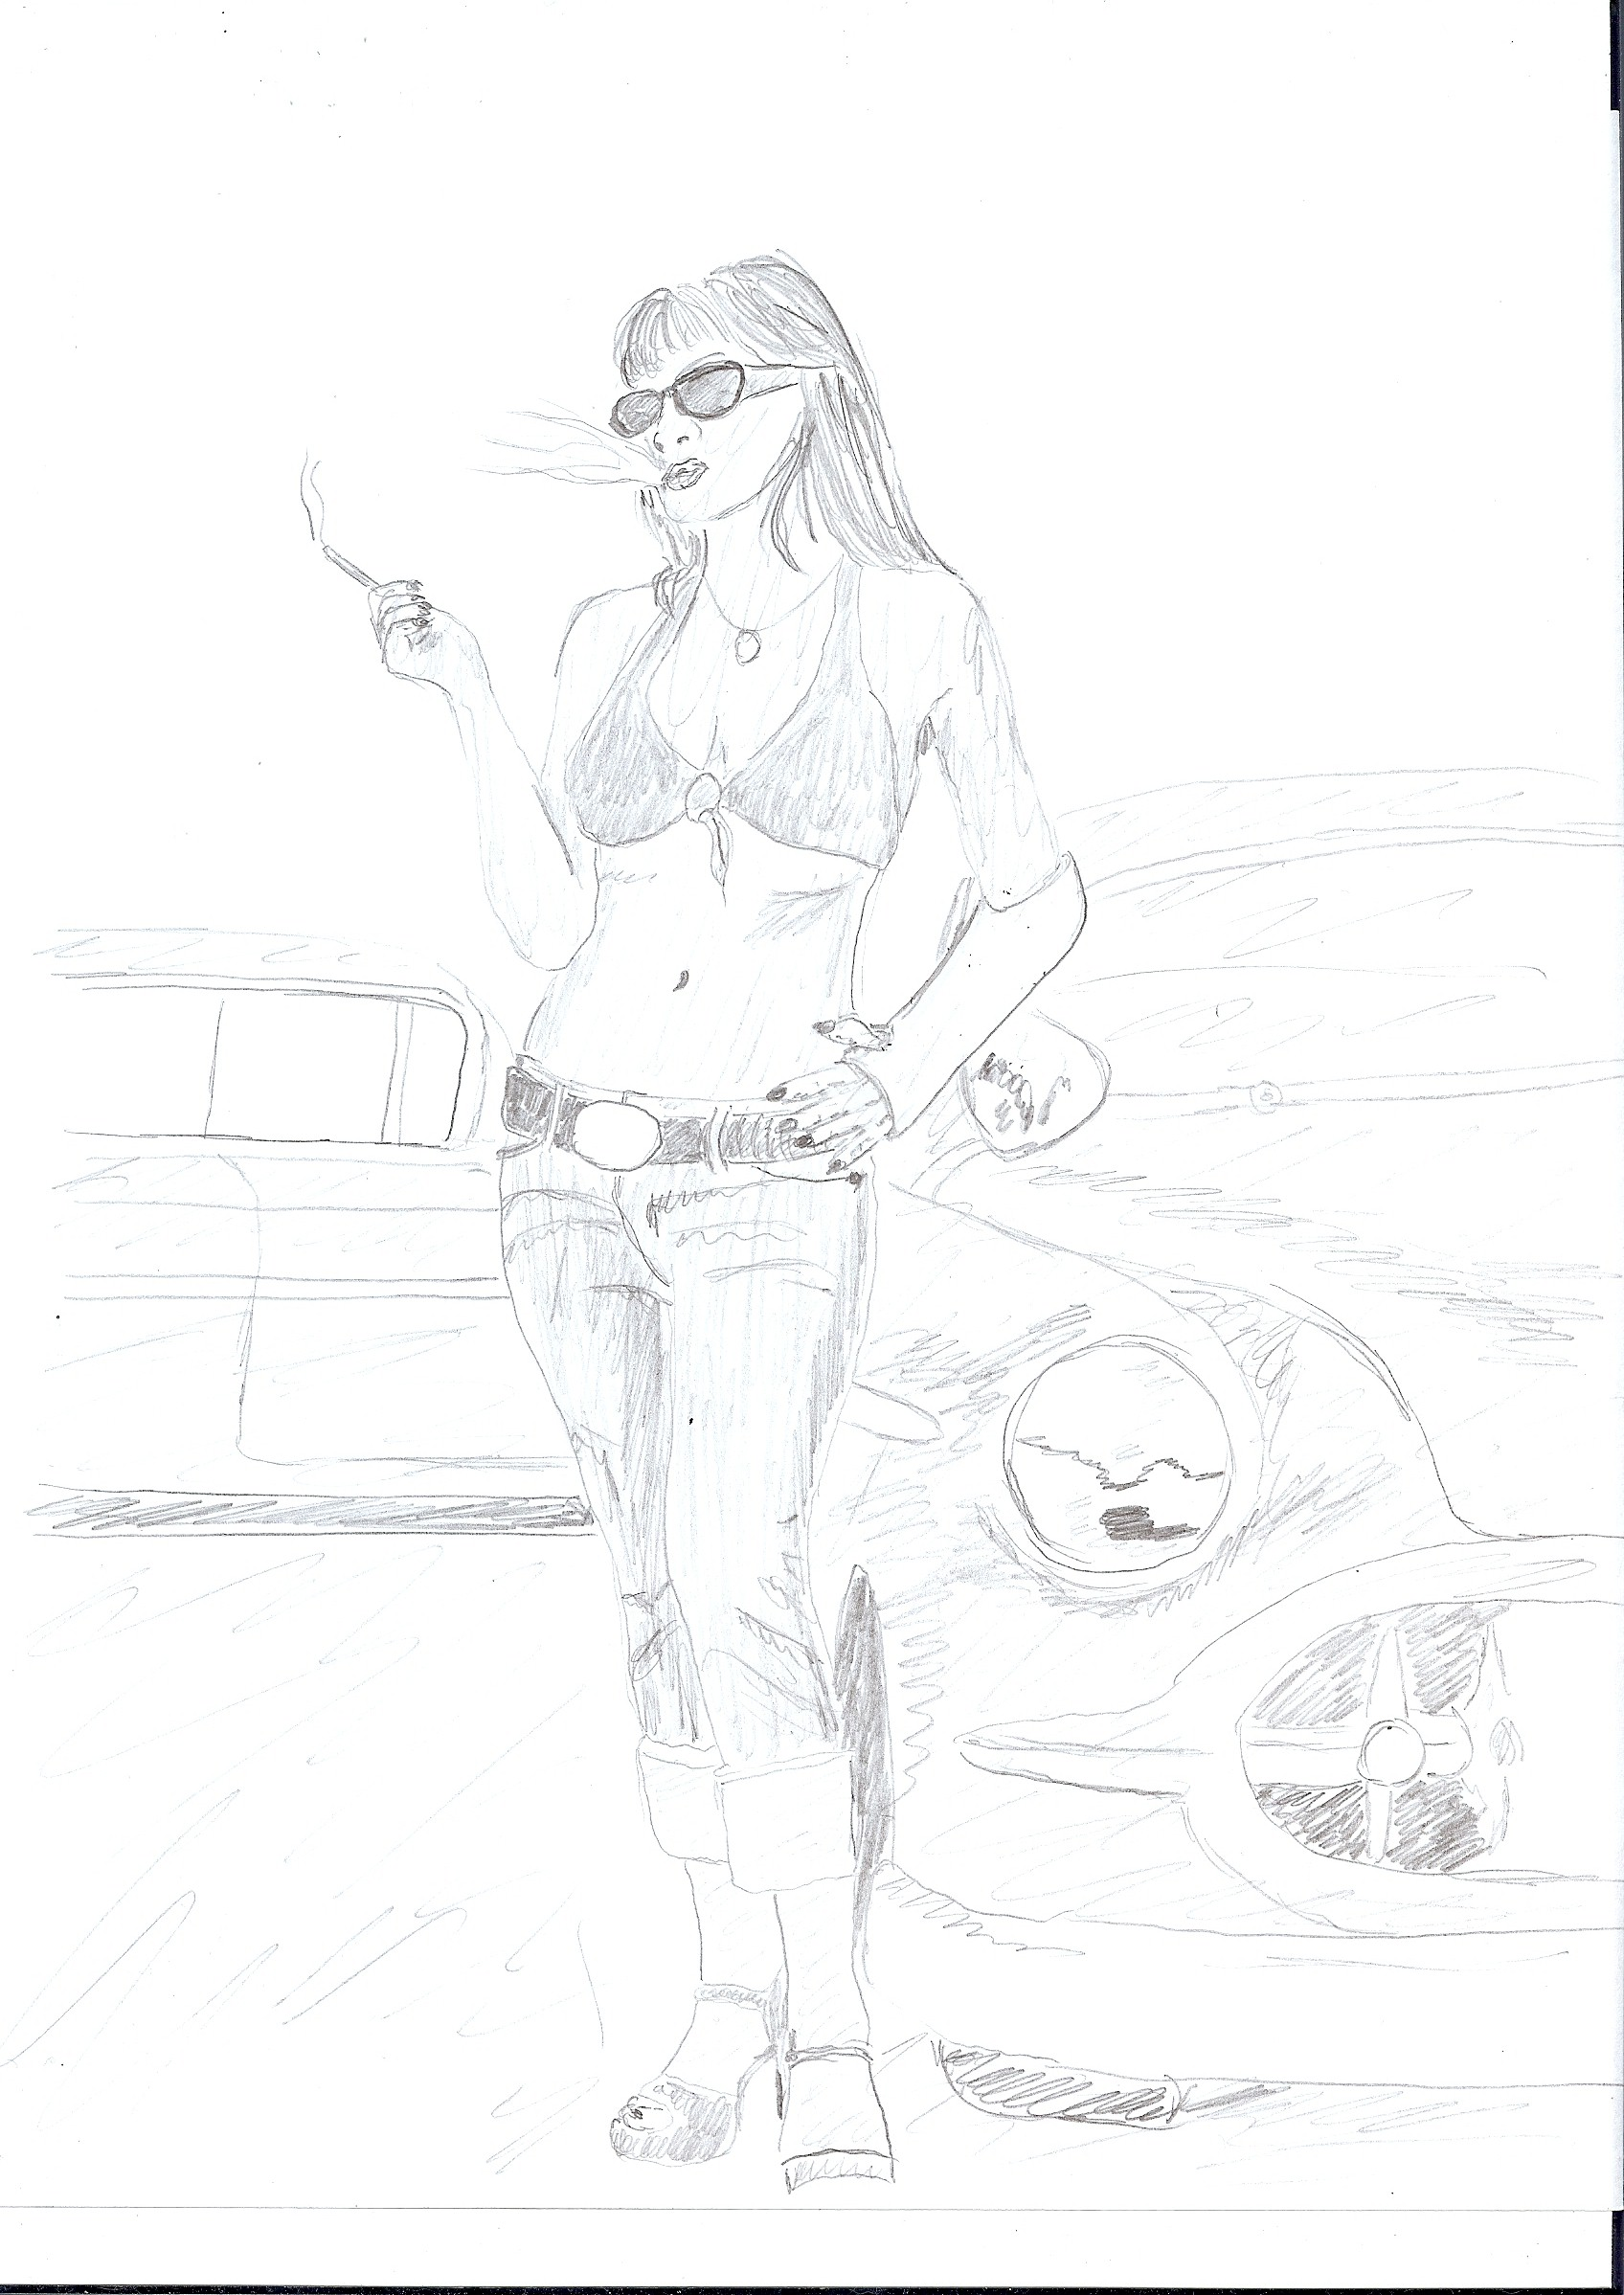
\includegraphics[height=0.8\textheight]{images/kicks50.jpg}
\end{center}
